\section{Wireless Bottleneck Detector}\label{Wireless Bottleneck Detector}

We strive to identify Home WiFi impairments, to achieve our goal we run experiments and trigger WiFi and non-WiFi issues in a testbed.  During our experiment sessions we collect active and passive metrics using a diverse set of tools. Most of the tools we work with are out-of-the-box tools, such as iPerf, tc and tcpdump. The active measurement tool we use to collect RTTs is a custom implementation of Ping in GoLang. We refer to this tool as \emph{GoPing}. We have customized GoPing to send ping trains and batches. These two features were key to find the probing rate we use for our experiments.

\subsection{Finding the probing rate}\label{probing_rate}

As described in section \ref{Back_Related_Work}, finding the probing rate is important when working with active measurements. A high rate can cause overhead, whereas a low rate can fail to capture the status of the network. To approach this challenge we conducted experiments in our office lab. Our experiments consisted in sending a series of ping trains which included multiple pings inside each train. We ran the tests with different train inter-spacing values and with different amount of pings inside the trains. The first finding from our experiments was a delay in RTT due to power save mode in devices. The power save mode sends the NIC to sleep. We refer to this delay as the ``sleeping NIC". We found that when the inter-train spacing is smaller or equal to 100 msec the power save mode delay is not present. Based on this finding we set our lower bound for inter-train spacing to 100 msec. We set our upper bound to 1000 msec as the RTT within a home WiFi single-hop network is expected to be only a few milliseconds without significant cross-traffic. This observation is remarked in the work of Sundaresan et al. \cite{homeoraccesslink}.

The second relevant finding is associated to the RTT value of each ping within a train. We found that even with inter-train spacing values above 100 msec it is possible to overcome sleeping NIC delay by considering the RTT value of the 3rd or greater ping within a train. We noticed that the RTT value for ping greater or equal to the 3rd ping in a train depicted similar RTT values as when the sleeping NIC delay is not present. After these observations we defined our baseline to be 100 msec inter-train spacing and 3 pings per train. Figure \ref{image:Avg_RTT_Three_Pings} illustrates the values for the average round trip time of three pings in a train. The inter-ping spacing is equally distributed among the number of pings in a train and the inter-train spacing. For example, the inter-ping spacing value for 3 pings in a 100 msec inter-train series is 100 msec/3 or ~33.33 msec.

\begin{figure}[h]
	\centering
	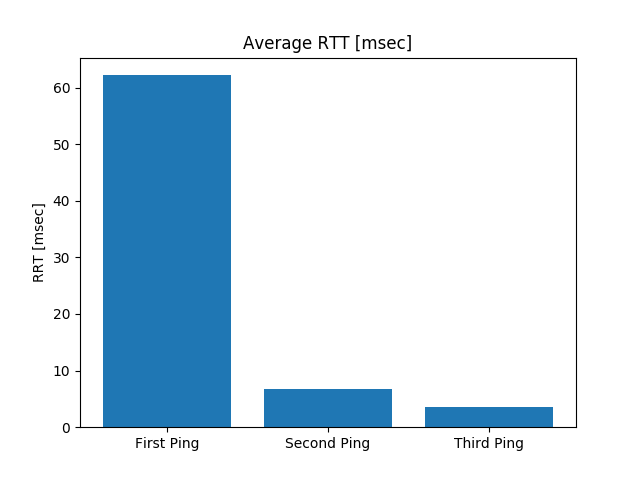
\includegraphics[width=8cm]{Three_Pings/Three_Pings_Avgs}
	\caption{Average RTT for Three Ping Series}
	\label{image:Avg_RTT_Three_Pings}
\end{figure}

With this exercise we defined our baseline, we implemented similarity tests between our baseline results and samples derived from the baseline. We refer to our baseline as aggressive probing. To keep the samples to follow the same distribution as our baseline we implemented a Poisson process to generate the inter-train space intervals. In other words, randomly sampling from a Poisson process will result in another Poisson-distributed process \cite{raikov_decomposition}. This feature has been included in our GoPing tool. We sampled our baseline to obtain from 10\% to 90 \% of our original data points. We implemented Bernoulli random sampling to extract our samples. Finally, we ran Two-sample Kolmogorov-Smirnov tests between our baseline and samples. From the results we noticed that the sample which delivers a similar ECDF to our baseline is the one that keeps 50\% of the original baseline data points. Figure \ref{image:ECDF_aggressive_vs_sampling} illustrates both ECDFs.

\begin{figure}[h]
	\centering
	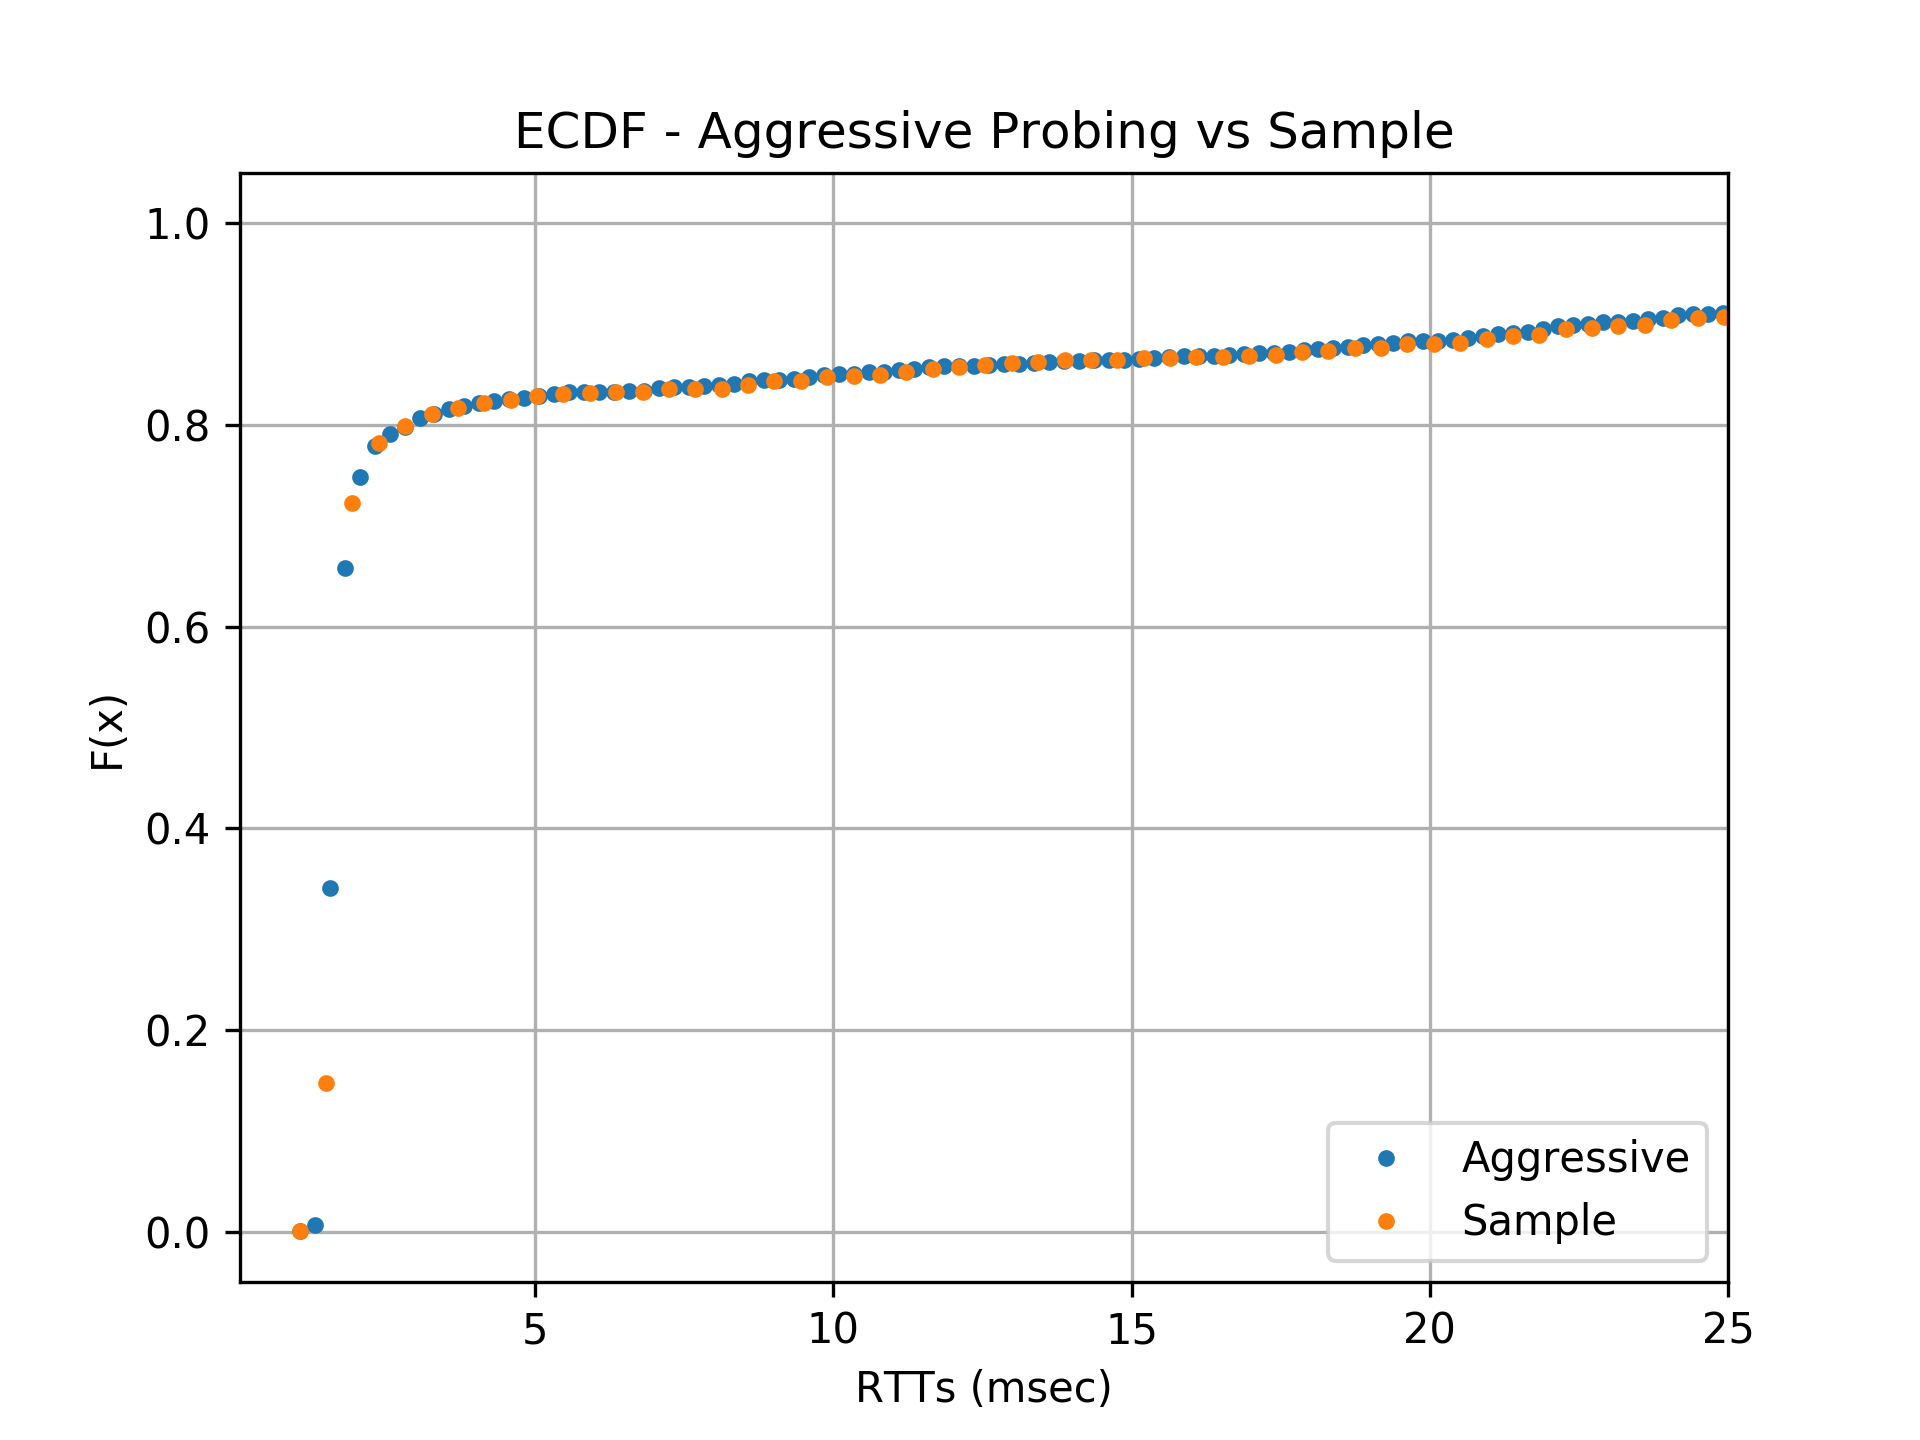
\includegraphics[width=8cm]{ECDF_Similarity/Aggressive_vs_Sample_Probing}
	\caption{ECDF - Aggressive Probing vs Sample}
	\label{image:ECDF_aggressive_vs_sampling}
\end{figure}

From figure \ref{image:ECDF_aggressive_vs_sampling} the overlap between the sample keeping 50\% of original data points and the original baseline derived from aggressive probing can be seen. This was the sample in which the overlap occurred, based on this result we obtained our probing rate. As the RTT ECDF of the sample with half of the original data is similar to the original baseline, we set our probing rate to be 200 msec. To validate our chosen probing rate still holds in our testbed we tested it. The tests consisted in sending as many batches as possible for 10 min at 100 and 200 msec probing rates. Additionally we varied the attenuation with values of 0, 15 and 30 dBm. Table \ref{table:Att_Rate_Test_Values} summarizes the values used for the test. The test sessions took place in the 2.4 GHz band using 802.11n WLAN with no authentication. We ran each experiment session 5 times, in total we obtained 30 samples.

\begin{table}[h]
\begin{center}
	\begin{tabular}{||c c||}
		\hline
		Attenuation & Probing Rate\\ [0.5ex] 
		\hline\hline
		0 dBm & 100msec\\ 
		\hline
		0 dBm & 200msec\\
		\hline
		15 dBm & 100msec\\
		\hline
		15 dBm & 200msec\\
		\hline
		30 dBm & 100msec\\
		\hline
		30 dBm & 200msec\\ [1ex] 
		\hline
	\end{tabular}
\end{center}
\caption{Attenuation and Probing Rate Validation Values}
\label{table:Att_Rate_Test_Values}
\end{table}

We compared the RTT ECDF of both rates as before to check similarity between probing rates. The expectation was for curves to be similar to each other. As expected, figure \ref{image:att_0_100and200msec} illustrates the similarity between both RTT ECDF probing rates.

\begin{figure}[h]
	\centering
	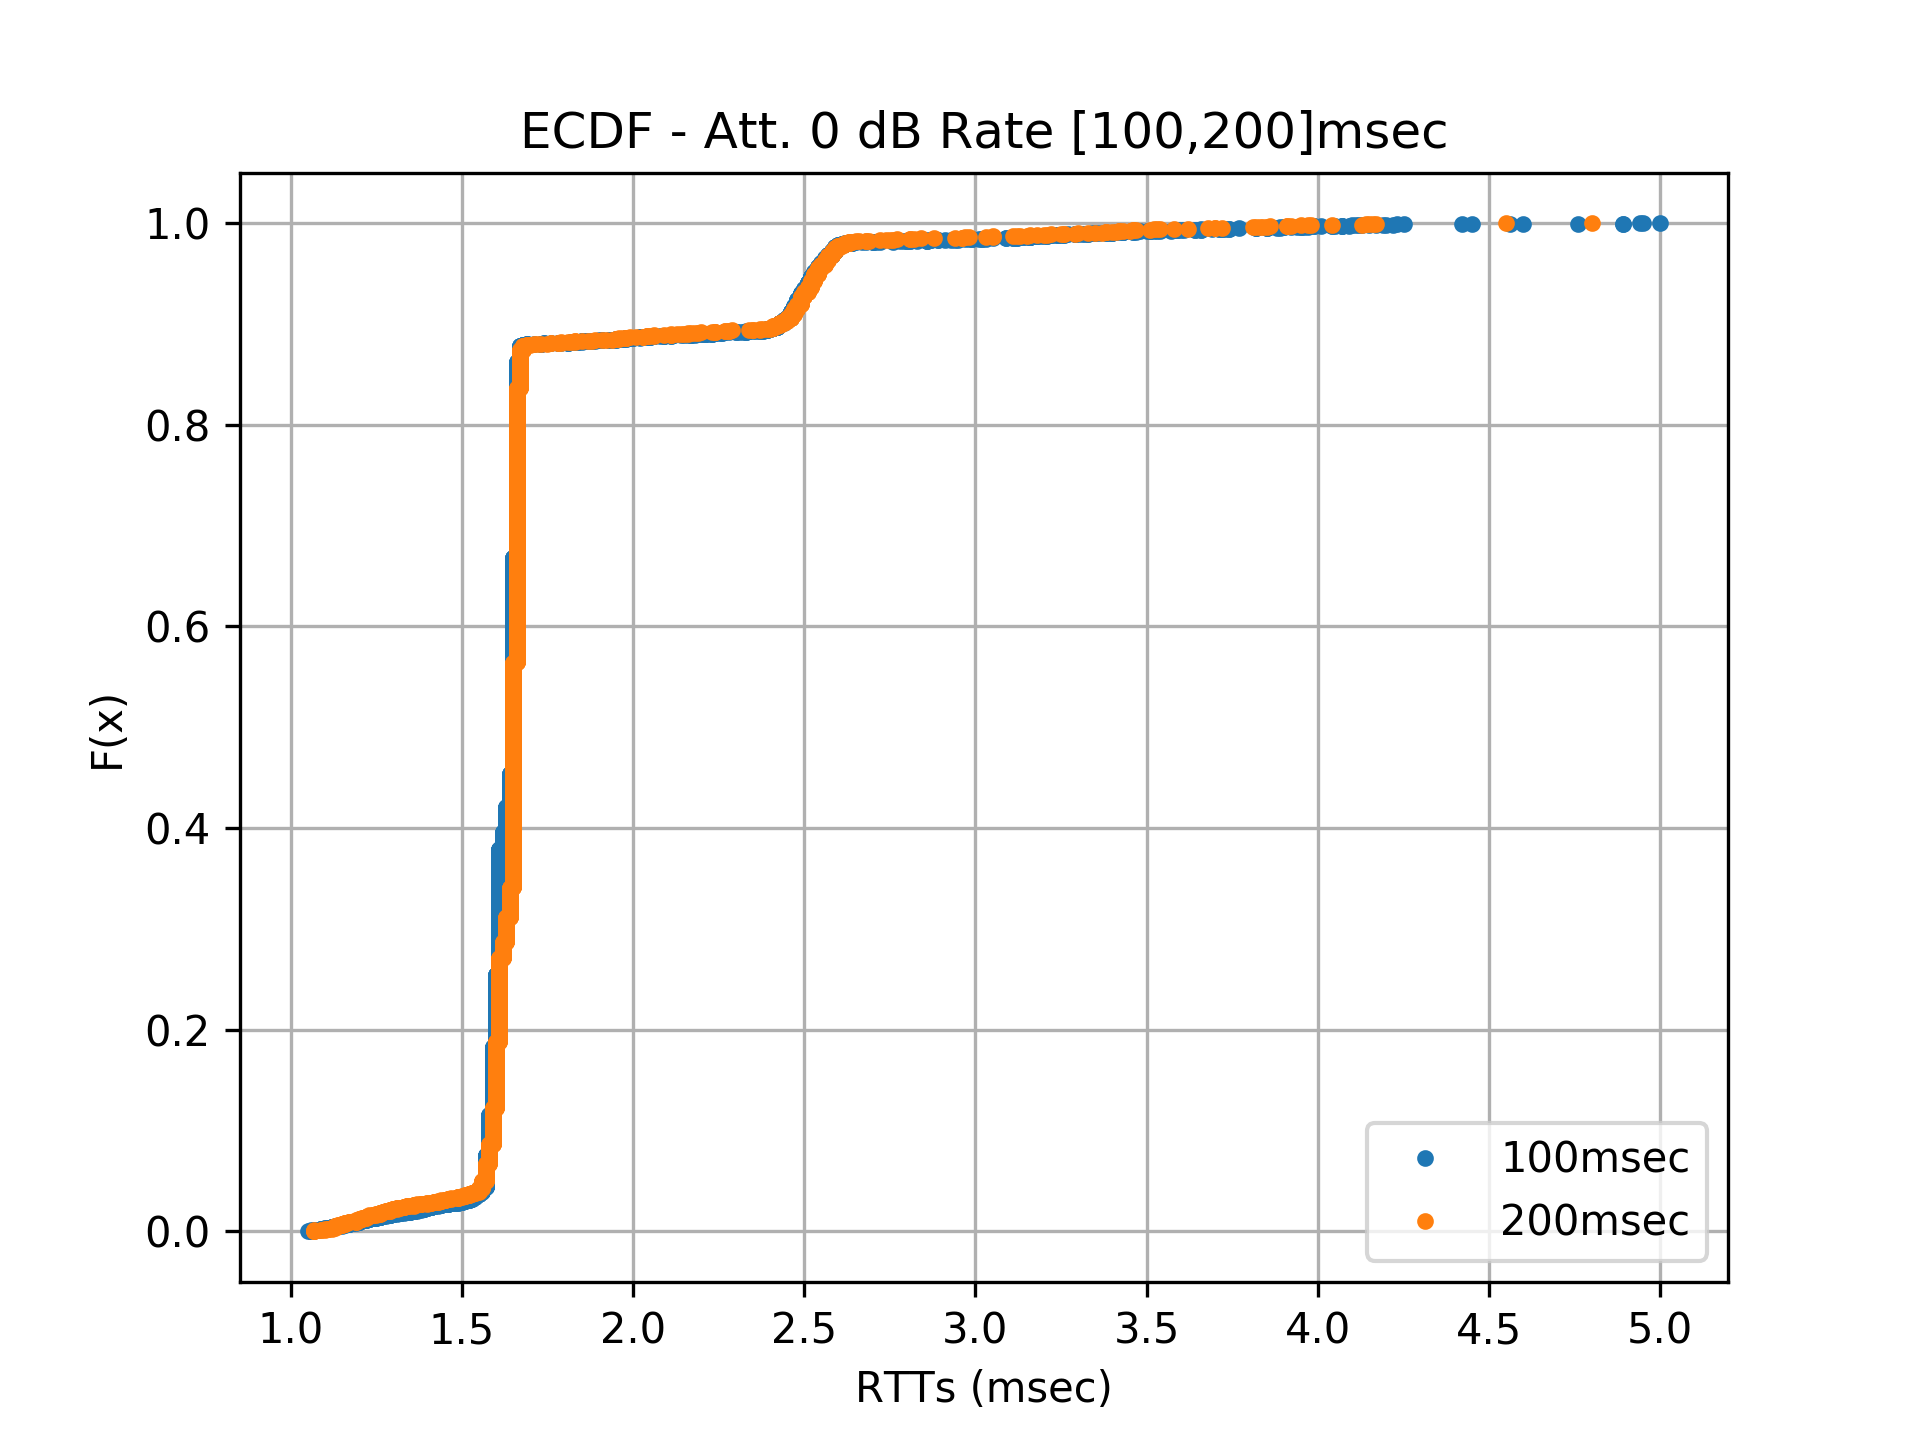
\includegraphics[width=8cm]{Rates_Atts/Att_0dBRate[100,200]msec}
	\caption{Att. 0 dBm - Rate 100,200 msec}
	\label{image:att_0_100and200msec}
\end{figure}

The next expected behavior was for RTT to increase as the attenuation values increases. Figure \ref{image:rate_200msec_Att_0_15_30dBm} help us to validate the expected behavior. As we increase attenuation, RTT increases.

\begin{figure}[h]
	\centering
	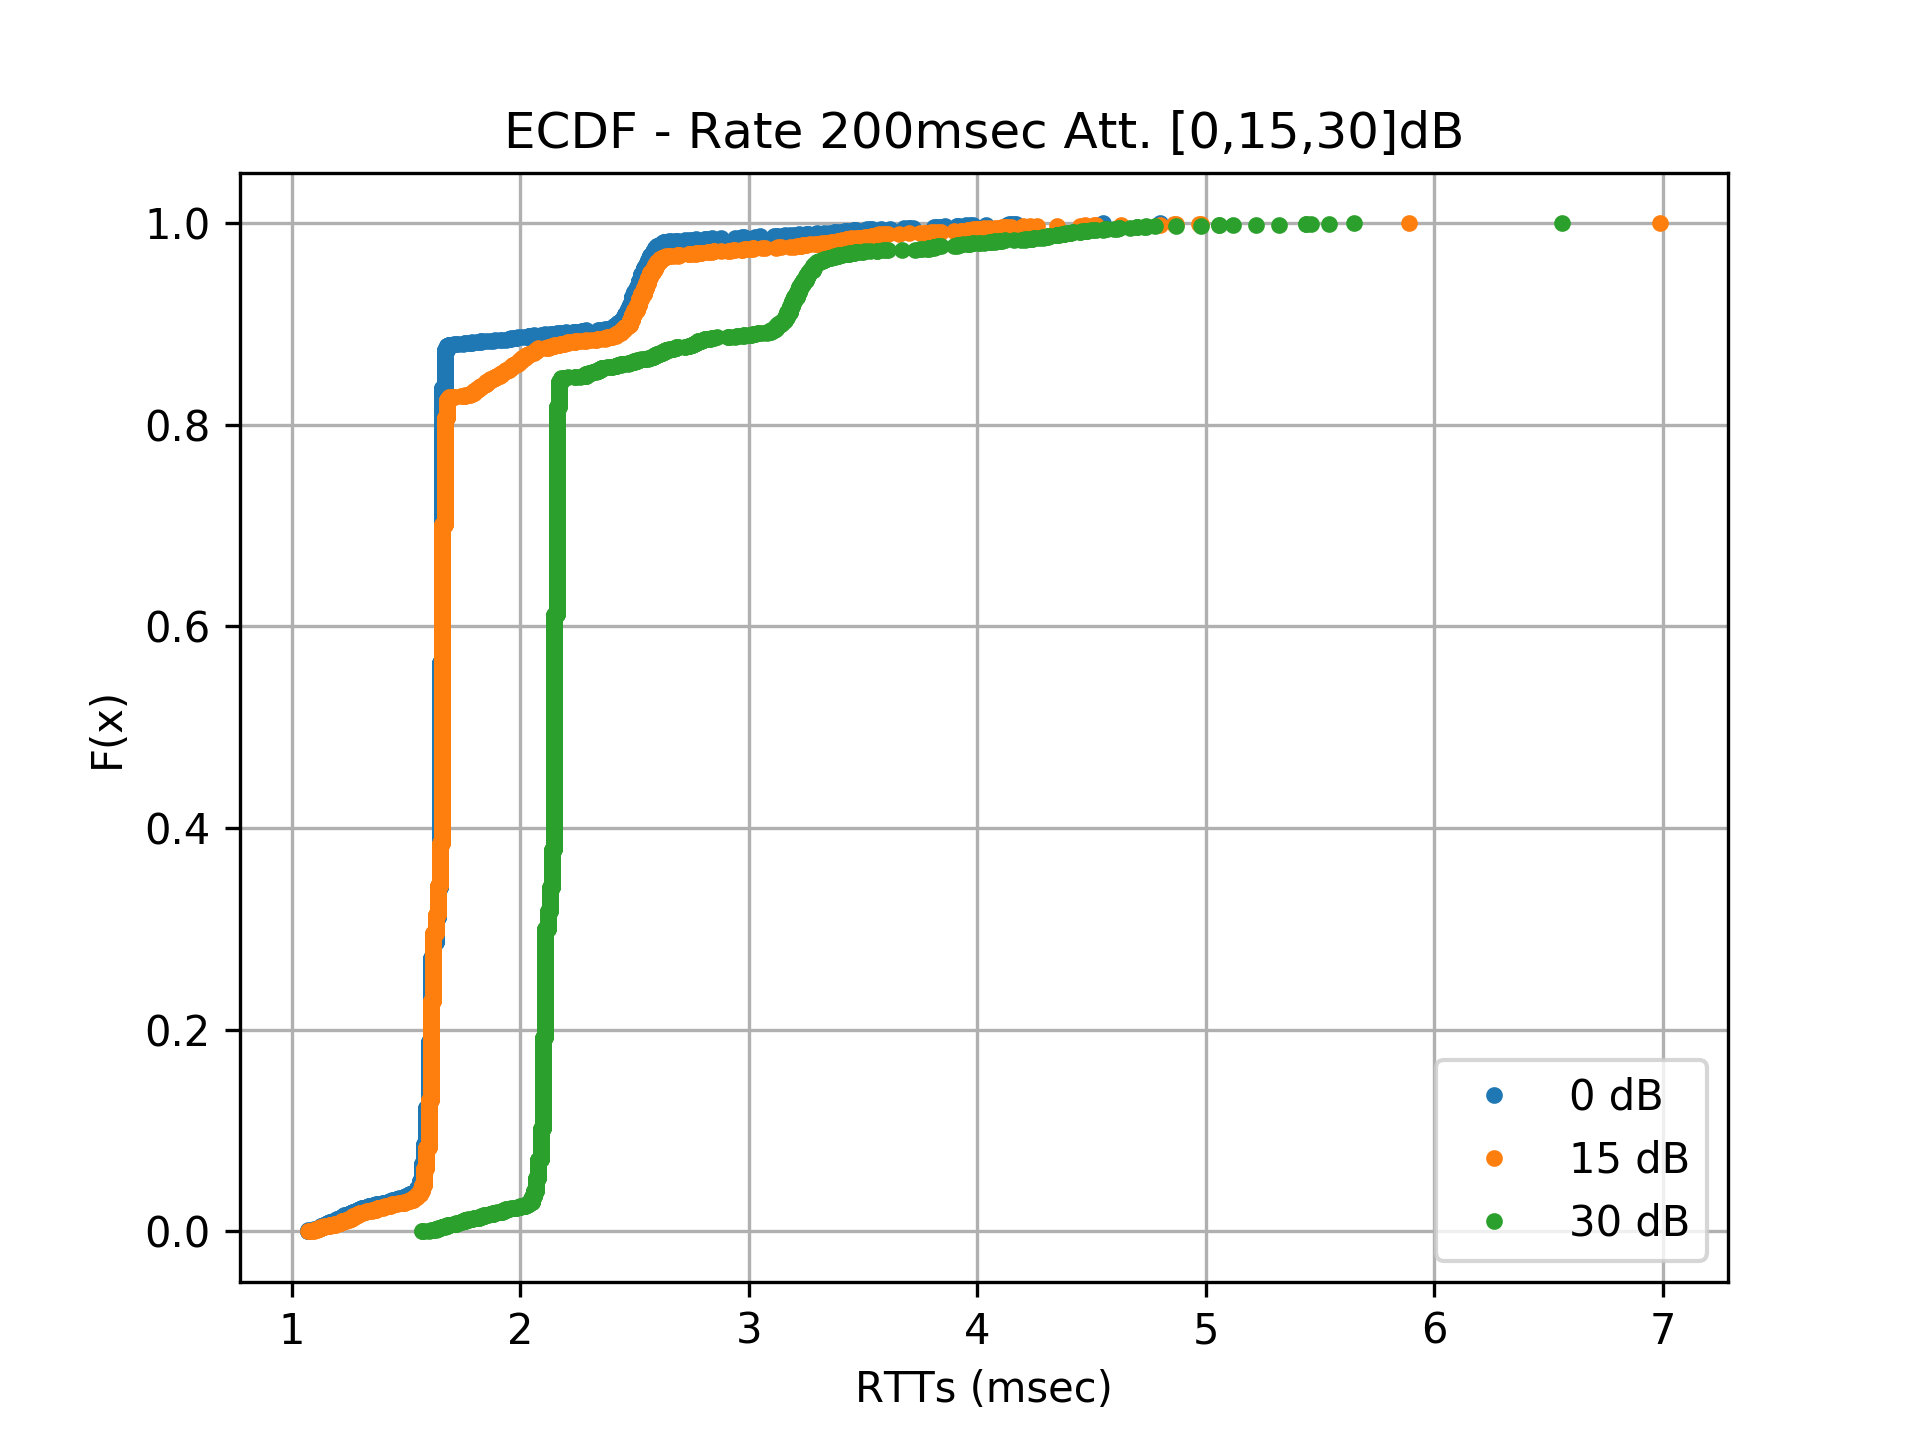
\includegraphics[width=8cm]{Rates_Atts/Rate200msecAtt_[0,15,30]dB}
	\caption{Rate 200 msec - Att. [0,15,30] dB}
	\label{image:rate_200msec_Att_0_15_30dBm}
\end{figure}